\documentclass{report}
\usepackage{titlesec}
\usepackage{titling}
\usepackage{graphicx}
\usepackage{tikz}
\usepackage{pgfplots}
\usepackage{caption}
\usepackage{multirow}


\title{\textbf{UBL201-L Introductory Biology III - Neurobiology}}
\author{Rahul Chavan - 22086}
\date{20th November 2023}


\usepackage[left=1in, right=1in, top=0.5in, bottom=0.5in]{geometry}
\renewcommand{\maketitle}{
 \begin{center}
    
\includegraphics[width=2cm]{IISc_Master_Seal_Black.jpg}
    \vspace{0.5cm}

    \Large
    \textbf{\thetitle}
    
    \vspace{0.5cm}
    
    \Large
    \theauthor
    
    \vspace{0.2cm}
    
    \large
    \thedate

    \vspace{0.5cm}

    \hrule  
    
  \end{center}
}

\pgfplotsset{compat=1.18}
\begin{document}
\maketitle
\begin{center}
    \Large
    \textbf{Neuronal Passive and Active properties}
\end{center} 


\subsection*{Question 1: V-I characteristics of a passive neuron }

\textbf{V-I characteristics of a passive neuron Given is a passive neuronal model where 
you can inject current pulses of different amplitudes. Measure the steady-state 
voltage response of the neuron in response to current pulses spanning the amplitude range 
of -500 to +500 pA (in steps of 100 pA). Plot steady-state voltage as a function of the 
current amplitudethat was used to elicit that deflection.}

\subsubsection*{Observations}

\begin{table}[!ht]
    \centering
      \caption{V-I characteristics of a passive neuron}
      \vspace{0.5cm}
      \label{tab:table1}
      
      \begin{tabular}{|c|c|}
        \hline
        \textbf{Current amplitude (pA)} & \textbf{Steady-State Voltage} \\
        \hline
        -500 & -133.62 \\
        \hline
        -400 & -120.93 \\
        \hline
        -300 & -108.197 \\
        \hline
        -200 & -95.4648  \\
        \hline
        -100 & -82.7324\\
        \hline
        0 & -70 \\
        \hline
        100 & -57.2676 \\
        \hline
        200 & -44.5352 \\
        \hline
        300 & -31.8028 \\
        \hline
        400 & -19.0704 \\
        \hline
        500 & -6.33802 \\
        \hline
      \end{tabular}
    \end{table}

\subsubsection*{Plot}
\begin{center}
    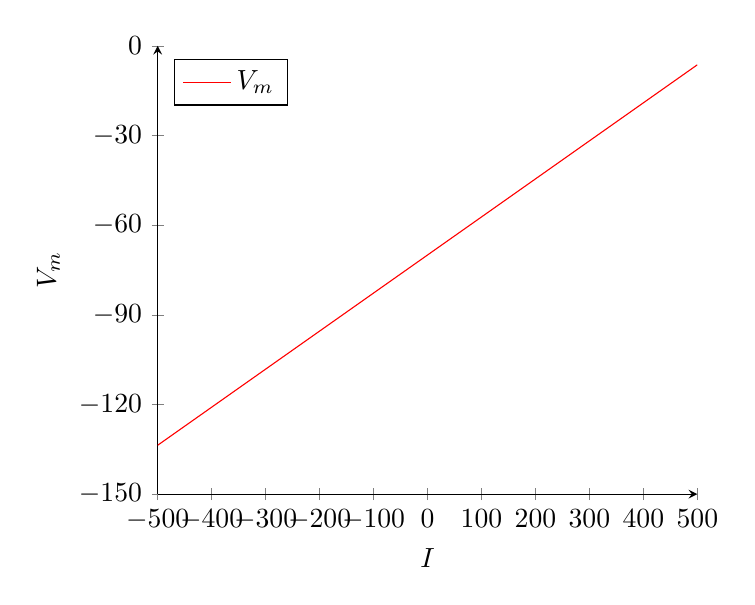
\begin{tikzpicture}
        \begin{axis}[
            axis lines = left,
            xlabel = $I$,
            ylabel = {$V_m$},
            xmin=-500, xmax=500,
            ymin=-150, ymax=0,
            xtick={-500,-400,-300,-200,-100,0,100,200,300,400,500},
            ytick={-150,-120,-90,-60,-30,0},
            legend pos=north west,
        ]
        \addplot [
            domain=-500:500, 
            samples=100, 
            color=red,
        ]
        {0.1273*x - 69.996};
        \addlegendentry{$V_m$}
        \end{axis}
    \end{tikzpicture}
\end{center}




\subsection*{Question 2: Ion Concentration vs. resting Membrane potential}
\textbf{Given is a neuronal model with only sodium and potassium leaky channels. 
Change the intracellular ion concentration of the following ions in the given range:
\begin{enumerate}
    \item Ca2+ : 1e-1 mM to 1e-5 mM (step size: 1e-1 mM)
    \item K+: 10 mM to 110 mM (stepsize: 20 mM)
    \item Cl-: 1 mM to 5 mM (stepsize: 1 mM)
    \item Na+: 10 mM to 50 mM (stepsize: 10 mM)
\end{enumerate}
Record the steady state resting membrane potential at each concentration. 
What do you observe for different ions? Can you derive the steady stateresting membrane 
potential value at the maximum concentration of each ion using the GHK equation?}

\subsubsection*{Observations for $Ca^{2+}$}

\begin{table}[!ht]
    \centering
      \caption{$Ca^{2+}$ concentration vs. Resting membrane potential}
      \vspace{0.5cm}
      \label{tab:table2}
      
      \begin{tabular}{|c|c|}
        \hline
        \textbf{$Ca^{2+}$ concentration (mM)} & \textbf{Resting membrane potential} \\
        \hline
        1.00E-01 &	-65.0829 \\
        \hline
        1.00E-02 &	-65.0829 \\
        \hline
        1.00E-03 &	-65.0829 \\
        \hline
        1.00E-04 & 	-65.0829 \\
        \hline
        1.00E-05 &	-65.0829 \\
        \hline
      \end{tabular}
    \end{table}

\subsubsection*{Observations for $K^{+}$}

\begin{table}[!ht]
    \centering
      \caption{$K^{+}$ concentration vs. Resting membrane potential}
      \vspace{0.5cm}
      \label{tab:table3}
      
      \begin{tabular}{|c|c|}
        \hline
        \textbf{$K^{+}$ concentration (mM)} & \textbf{Resting membrane potential} \\
        \hline
        10 &	-65.0829 \\
        \hline
        30 &	-65.0829 \\
        \hline
        50 &	-65.0829 \\
        \hline
        70 & 	-65.0829 \\
        \hline
        90 &	-65.0829 \\
        \hline
        110 &	-65.0829 \\
        \hline
      \end{tabular}
    \end{table}

\subsubsection*{PLOT}
\begin{center}
    \begin{tikzpicture}
        \begin{axis}[
            axis lines = left,
            xlabel = $[K^+]$,
            ylabel = {$V_m$},
            xmin=0, xmax=120,
            ymin=-150, ymax=0,
            xtick={0,20,40,60,80,100,120},
            ytick={-150,-120,-90,-60,-30,0},
            legend pos=north west,
        ]
        \addplot [
            domain=0:120, 
            samples=100, 
            color=red,
        ]
        {-65.0829};
        \addlegendentry{$V_m$}
        \end{axis}
    \end{tikzpicture}
\end{center}









\end{document}